\chapter{Einleitung}\label{ch:einleitung}
Vor mehr als fünfzig Jahren wurde der allererste Großrechner, auch Mainframe genannt, vorgestellt.
Seit dieser Zeit setzen sich die monolitisch aufgebauten Systemes im Bezug auf Leistungsfähigkeit und Zuverlässigkeit gegenüber andere Systeme ab.
Obwohl die Systeme immer weniger Platz brauchten, anfangs waren es ganze Gebäudestockwerke, heute sind es ungefähr die Ausmaße eines großen Kleiderschrankes.
Und weiteren Verbesserung bei der Handhabbarkeit, von reinen Druckausgaben über text-basierenden Terminals bis hin zu benutzerfreundlichen GUI´s.
Auch hat sich die Weise, wie Programme entwickelt werden verändert.
Zu Beginn mussten diese noch auf Lochkarten (ABBILDUNG !!) gestanzt und umständlich über ein Lesegerät eingelesen werden.
Heute stehen dem Entwickler moderne IDE´s zur Verfügung.
Trotz dieser Veränderungen verlor der Mainframe durch die Dezentralisierung der IT hinzu Client-Server-Umgebungen in den 1990-er Jahren an Bedeutung.
Dieser Prozess führte soweit, dass in den frühen 1990-er Jahren bereits Vorhersagen über die Abschaltung des letzten Mainframes getroffen wurden. \footnote{\cite{Alsop.1993}}
\cite{Ceruzzi.2003}

Trotz dieser Vorhersagen verarbeiten heutzutage Großrechner weltweit circa 1,2 Millionen CICS\footnote{Begrifferklärung zu CICS in \ref{cics}} Transaktionen pro Sekunde.\footnote{\cite{IBM.2019}}
Im Vergleich hierzu werden 63.000 Google Suchanfragen pro Sekunde abgesetzt. \footnote{\cite{Sullivan.2016}}
Wie hat es diese schon seit den frühen 1990-er Jahren totgesagte Technologie geschafft auch heute noch diese Relevanz zu haben?
Hier kommen die klar definierte Vorteile und Use-Cases des Mainframes zum tragen.
Zunächst ist `RAS`\footnote{reliability, availability and serviceability} zu nennen.
Dies beschreibt grundsätzlich, die Stabilität eines Hard- und Softwaresystems.
Hierzu zählt vor allem das Verhalten bei einem Hardware-/Softwaredefekt und möglichst automatische Erkennung und möglichst effektive Behebung von diesem.
Zusätzlich sollte dies keinen oder nur selten einen kompletten Systemausfall zur Folge haben.
\begin{figure}[h]
	\centering
	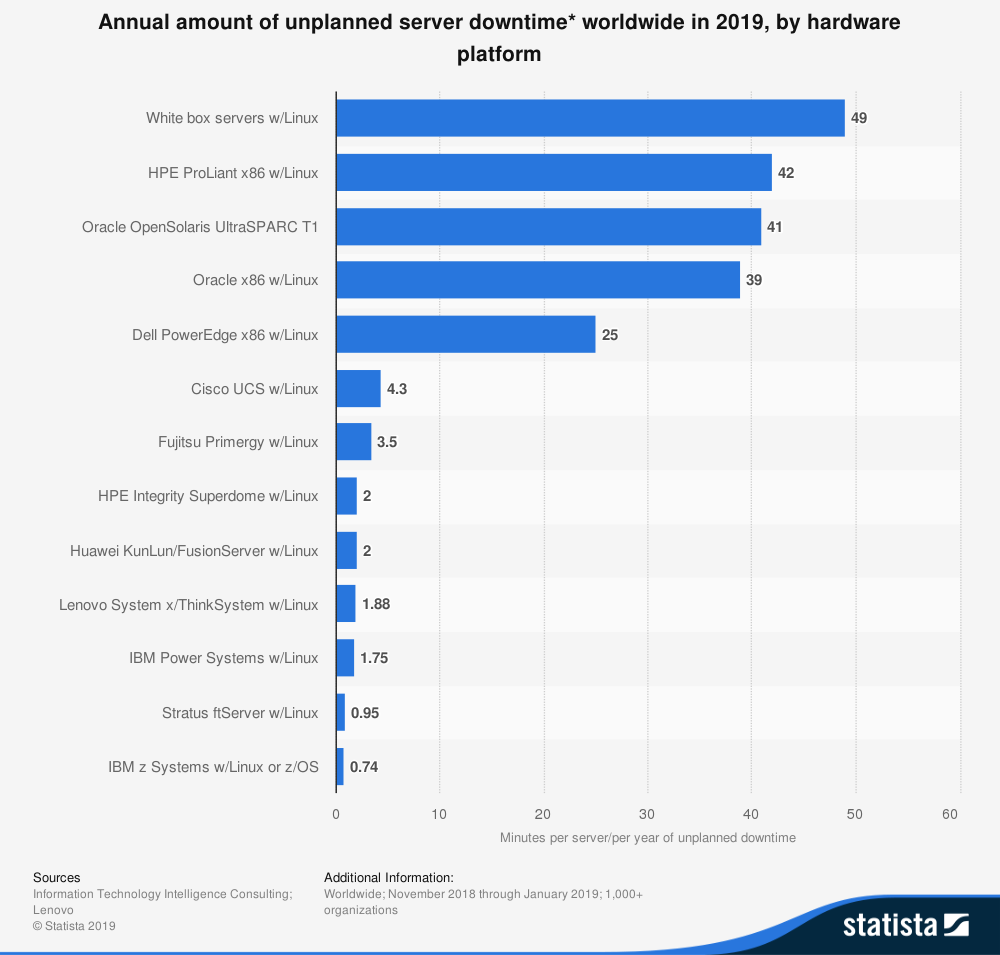
\includegraphics[width=\textwidth]{figures/statistic_id515285_unplanned-server-downtime-globally-2019-by-hardware-platform.png}
	\caption{Annual amount of unplanned server downtime worldwide in 2019, by hardeware platform}
	\label{fig:serverdowntime}
\end{figure}
Abbildung \ref{fig:serverdowntime} zeigt die ungeplannte Server Ausfallzeit in Minuten pro Server im Jahr 2019.
Wie zu sehen ist, schneidet der IBM z Systems w/Linux oder z/OS, das Mainframesystem der IBM, am besten ab.


Hinzu kommen spezielle Sicherheitsmechanismen und Skalierbarkeit.
All dies verbunden mit der durch (HIER SPECS EINFÜGEN) gewehrleisteten Performance, ermöglicht spezielle Use-Cases.
Unteranderem Massendatenverarbeitung, die dazugehörige Resourcenverwaltung und Breitband Kommunikation.
Das macht den Mainframe vor allem für Banken, das Gesundheitswesen, Versicherungen, Fluggesellschaften usw. attraktiv.
Zu diesen Unternehmen zählt auch die DATEV eG.
\cite{IBM.2014}

Die DATEV eG wurde am 14.02.1966 von 65 Steuerbevollmächtigten gegründet.
Sie verfolgten das Ziel Buchführungsaufgaben mit Hilfe der EDV zu bewältigen.
Aufgrund hohen Mitgliederwachstums wurde hierfür 1969 in einen firmeneigenen IBM-Großrechner investiert.\cite{DATEVeG.2017}
Bis heute läuft ein nicht unbeträchltlicher Teil der betriebswirtschaftlichen Anwendungen auf einem IBM-Mainframe.
Darunter fallen circa 14.000 aktive Module.


Was ist der Mainframe\\
Geschichte\\
kurzer technischer Einblick Mainframe und Vorteile und (Bedeutung bei Datev) \\
wieso er bei Datev eingesetzt wird \\
 Moma \\
 Problemstellung \\
 Wieso Rechnungsschreibung als Beispiel? \\